\chapter{A highland maize chromosomal inversion decreases flowering time in a phosphorus-independent manner and leads to a minor perturbation of the leaf phosphorus starvation response transcriptome.}
\label{chap-three}
\newrefsection

\section{Abstract}
\invfour is a chromosomal inversion commonly found in traditional maize varieties grown in the Mexican highlands. 
\invfour was introgressed into cultivated maize from highland teosinte mexicana, and its highland predominance points to its contribution to local adaptation. 
In growth chamber experiments, \invfour-highland has been shown to regulate the expression of photosynthesis genes in response to cold.
In addition to cold, phosphorus is a limiting factor for plant growth in the Mexican highlands. 
In this study, we tested whether \invfour-highland contributes to local adaptation through an enhanced response to phosphorus deficiency. 
First, we bred Near Isogenic Lines (NILs) in B73 containing \invfour-highland introgressed from MICH21, a traditional Mexican maize variety, with the purpose of isolating the effect of \invfour-highland in a single, common genetic background.
Then we grew the \invfour-highland and control lines in the field under phosphorus sufficiency and deficiency. 
We measured flowering time, morphological traits, and leaf gene expression with RNA-seq. We found that independent of soil phosphorus status, \invfour-highland NILs flowered faster and grew taller than the controls while maintaining grain yield. 
There was a genomewide transcriptomic response to available phosphorus, affecting 7373 differentially expressed genes (DEGs), with the largest effect shown by \textit{PILNCR1-miR399}, a PSR regulator. The effect of \invfour-highland is narrower, affecting 528 DEGs, mainly within the boundaries of the inversion. The \invfour perturbation of PSR is limited to 1 DEG, the putative aldehyde dehydrogenase \textit{aldh2}. 
Our results confirm the contribution of \invfour to adaptation, as faster flowering, but we don’t find evidence of its effect on PSR.

\section{Background}

Chromosomal inversions might contribute to local adaptation by capturing locally adapted genotypes of several loci and limiting subsequent recombination \citep{kirkpatrick2006b}. 
In a Mexican diversity panel of maize traditional varieties (TVs), a chromosomal inversion in the chromosome 4, \invfour, was associated both to elevation and flowering time \citep{romero_navarro2017-cn}. 
More specifically, \invfour shows a classical pattern of gene-by-environment interaction produced by local adaptation: plants with the \invfour-highland allele have delayed flowering at low elevations and earlier flowering at high elevations \citep{crow2020}. 
The highland haplotype of \invfour was introgressed from \textit{Zea mays spp.} \mex \citep{calfee2021-mr,gonzalez-segovia2019-jy,hufford2013-gs} which is a maize wild relative native to the Mexican highlands. 
The \invfour inversion spans 13 Mb \citep{pyhajarvi2013, calfee2021-mr}, shows recombination repression, low genetic diversity, has clinal dependency on elevation, and is almost fixed at locations higher than 2500 m.a.s.l (\autoref{fig::design} A and B), \citep{crow2020,gonzalez-segovia2019-jy}. 
In a precedent work, \citep{crow2020}, \invfour-highland was shown to up-regulate the expression of photosynthesis genes in response to cold in seedlings. 
But cold is not the only limiting factor for plant growth in the highlands.
Andosols are volcanic soils that are almost exclusive to the highlands, in Mexico 95\% of natural andosols profiles are present above 2000 m.a.s.l, (calculated from \cite{paz-pellat2018,inegi2013}). 
Due to their vitreous nature andosols have high phosphorus retention, \citep{krasilnikov2013}, and tend to have low amounts of phosphorus available for plant uptake, \citep{galvan-tejada2014}.
MICH21 one of the accessions tested by \citep{crow2020}, is native to the Purépecha Plateau, where both, andosols \citep{paz-pellat2018,inegi2013,galvan-tejada2014}, and phosphorus use efficient maize TVs are usual \citep{bayuelo-jimenez2011, bayuelo-jimenez2014}. 
\invfour might contribute to faster growth in the highlands by carrying alleles that are beneficial during phosphorus starvation response (PSR).
In this study, we investigate whether \invfour-highland contributes to local adaptation through an enhanced response to phosphorus deficiency.
Here we use a more advanced generation of the Mi21-derived sub-population assyed by \citep{crow2020} for testing the effect of \invfour in the gene expression response to cold.

\begin{figure}[!ht]
\centering
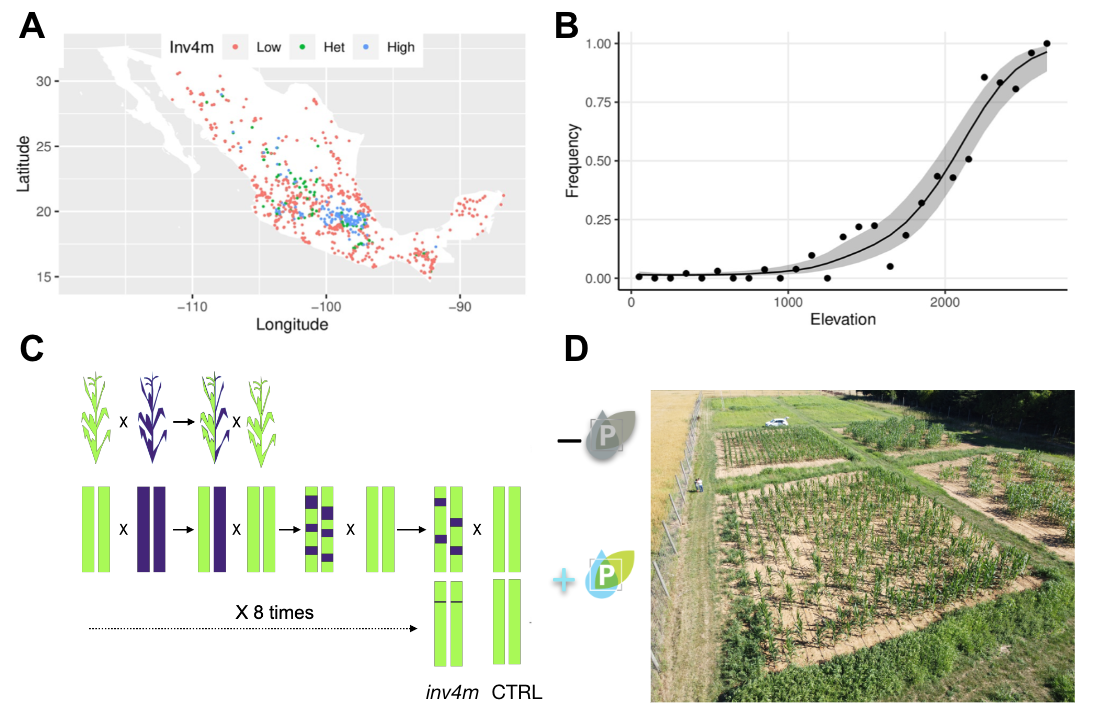
\includegraphics[width=\linewidth]{Chapter-3/figs/design.png}
\caption[\textit{\invfour} Distribution and Introgression Breeding Design]{\textit{\textbf{\invfour Distribution and Introgression Breeding Design.}} [A and B reproduced from \cite{crow2020}] \textbf{(A)} Distribution of lowand homozygous (Low), heterozygous (Het), and highland homozygous individuals of \invfour in Mexican traditional varieties.
\textbf{(B)} \invfour Allele Frequency Cline with Elevation in 100m bins.
\textbf{(C)} Near Isogenic Line breeding scheme, see details in methods, lines in the experiment are BC$_6$S$_2$.
\textbf{(D)}  Rock Springs, Pa, field station experimental setup.
}
 \label{fig::design}
\end{figure}

\section{Methods}
\subsection{\invfour plant population, growth conditions, experimental design, and phenotype measurements}

To measure the effects of the \invfour in plant field phenotypes and their phosphorus starvation response transcriptome, we used a highland traditional variety carrying the Highland haplotype of \invfour corresponding to the inverted karyotype.
The accession Michoacán 21 (referred to as Mi21), from the Mexican Cónico group, was obtained from the International Maize and Wheat Improvement Center (CIMMYT). 
In contrast, the reference genome of the temperate inbred B73, the recurrent parent for introgression, carries the lowland haplotype corresponding to the standard non-inverted karyotype at \invfour.

From the cross of Mi21 with B73 one F1 individual was backcrossed to B73 for six generations. During each cycle, we selected lines carrying  \invfour with a diagnostic SNP using a cleaved amplified polymorphic sequence (CAPS) marker. 
The marker SNP is PZE04175660223 located at position 4:181637780 in the NAM v5 \textit{Zea mays} genome assembly.
Amplification of the polymorphic site was done with the following primer pair: CTGAGCAGGAGATGATGGCCACTC and GGAAAGGACATAAAAGAAAGGTGCA, and subsequently cleaved by \textit{HinfI}.
Plants were genotyped using the CASP marker for selecting heterozygous plants at BC6S2 after selfing seeds of \invfour and CTRL homozygous individuals were selected for the field trial.


Plants were planted on May 26 2022 at the Russell E. Larson Agricultural Research Farm in Rock Springs, Pennsylvania (40°42’36" N 77°57’0" W, 366 m.a.s.l.) in soil classified as a Hagerstown silt loam (fine, mixed, semiactive, mesic Typic Hapludalf).
Experimental conditions were similar to previously described \citep{strock2018}. 
The experiment had a complete block design with two phosphorus (P) levels. 
Low-P fields (5 ppm Melich-3 Phosphorus)  and  high-P fields (36 ppm Melich-3 Phosphorus) were divided into smaller blocks. 
Three rows per block were planted with a mean stand count of 8 plants per plot, and the plants from the center row were selected for measurements to avoid border effects. Fields received fertilization based on treatment requirements. 
Drip irrigation was provided during dry periods. 
Each genotype was replicated four times within its P treatment.


\subsection{Phenotype analysis}

For stover mass growth curves, a different plant at each time point 40, 50, 60, and harvest, 121 days after planting (DAP), was collected, dried, and weighed for the same row. Stover dry mass data was fitted to a logistic growth model using the R package `growth curves`.
Maximum Stover dry weight was estimated to be the maximum over the four time points and not dry weight at harvest.
Ear measurements were taken for one ear per row at harvest. 

Phenotypes were modeled with thee R `lm` function as a multivariate multiple regression with fixed effects in the form of:

$$Y_{ijk} = \mu+ \beta_{1}C_{ijk} + \beta_{2}P_j+ \beta_{3}  \text{\invfour}_k+ \beta_{4} [\text{P} \times \textit{\text{\invfour}}]_{ij} + e_{ijk}$$.

with 

$$e_{ijk}\sim \mathcal{N} (0, {\sigma}^2)$$

For each phenotype $Y$, we modeled a response from the covariates $C_{ijk}$, that include row, column and block, $P_{i}$  the phosphorus treatment, $\text{\invfour}_{j}$ the \invfour genotype,  $[\text{P} \times \textit{\text{\invfour}}]_{ij}$ the genotype by treatment interaction term, and $e_{ijk}$ the residual for each replicate $k$, normally distributed with  mean zero and  variance $\sigma^2$.
Multiple hypothesis correction for the  t-test of model coefficient was done with a false discovery rate (fdr), and significant effects were reported below fdr = 0.05. 

\subsection{RNAseq tissue sampling, RNA extraction and Sequencing}
We took tissue samples 63 DAP when plants were between v7 to v9 developmental stages. 
Ten disc samples from the first leaf with a fully developed collar and every other leaf below for a total  of  four sampled leaves   per plant which where numbered 1-4 from apical to basal (\autoref{fig::RNAseq} A). 
Tissue was fast frozen in 1.5 mL tubes with two steel beads precooled with liquid nitrogen and kept in dry ice until stored at -80oC.
Four replicate plants were sampled per combination of  P treatment and \invfour genotype for a total of 64 tissue samples. 
I extracted total RNA with QIAGEN RNAeasy Plant Mini Kit  RNA extraction kit following manufacturer procedures (QIAGEN 74904), and RNA samples were quantified in nanodrop and sent to the NCSU Core Genomics Facility.
Following QC in bioanalyzer, Illumina libraries were prepared and sequenced in a lane of Novaseq according to manufacturer recommendations.


\subsection{Differential Gene Expression Analysis}
I aligned reads to the maize B73 NAM v5 genome using Kallisto \citep{bray2016}.
The alternative transcript alignment was turned into counts per gene per MB. We then used  voom  to calculate variance according to gene expression levels and counts were converted to log2(CPM). Then a  multivariate multiple regression between expression was run on each of the leaf positions, using the following model in limma :

$$Y_{ijk} = \mu + \beta_1 P_{ij}+ \beta_2 \text{\invfour}_{ij}+ \beta_3 [\text{P} \times \textit{\text{\invfour}}]_{ij} + e_{ijk}$$

with 

$$e_{ijk} \sim \mathcal{N} (0,\phi\sigma^2)$$

Linear model coefficients t-test p values were adjusted as false discovery rates, genes whose effect had a fdr <0.005 were deemed to be differentially expressed.
R scripts and expression data are  available at the  \href{https://github.com/sawers-rellan-labs/inv4mRNA}{\texttt{inv4mRNA} github repository}.



%\subsection*{Gene Regulatory Network Analysis}

%\subsection*{Lipid Analysis}



% \subsection{Phosphorus response of the leaf gene regulatory network to \invfour introgression}

\section{Results}

\subsection{Vegetative and reproductive traits had a marked response to phosphorus treatment and \invfour, but there is no  \invfour $\times$ P interaction effect}

I found a clear phenotypic response to phosphorus treatment independently of \invfour genotype ($\beta$ t-test, $\textrm{fdr} < 0.05$ ). 
Plants grown in low phosphorus grow slower and reach maturity later, with a similar effect in both \invfour and CTRL plants (\autoref{fig::effects} A). 
The effect of phosphorus treatment is significant for all the vegetative growth measurements taken, plant height at anthesis, and dry mass at 40, 50, 60, and 120 DAP.  
Plants growing in low phosphorus had faster male and female flowering times, greater cob width and length, and a reduced yield as measured by total kernel weight per ear (\autoref{fig::effects} B).
A closer analysis of the growth curves inferred from accumulated dry mass on different days showed an increased maximum stover dry mass in high phosphorus conditions, a faster mass acquisition rate, and a shorter time to mid-mass in higher phosphorus (\autoref{fig::growth}). 
There is slight evidence for an interaction between \invfour karyotype and growth. 

In a phenotype PCA of the different mean row trait values the first dimension explains 28\% of the variance. with morphological phenotypes has weights associated with flowering time and dry mass accumulation, highlighting these variables as the most responsive to the phosphorus treatment (PCA biplot). 
The samples in this phenotypic space show a clear separation by treatment but not  \invfour karyotypes ( 2 x MANOVA 2 groups F test, p < 0.05) or their interaction (MANOVA 4 groups, F test, p > 0.05).


\begin{figure}[!ht]
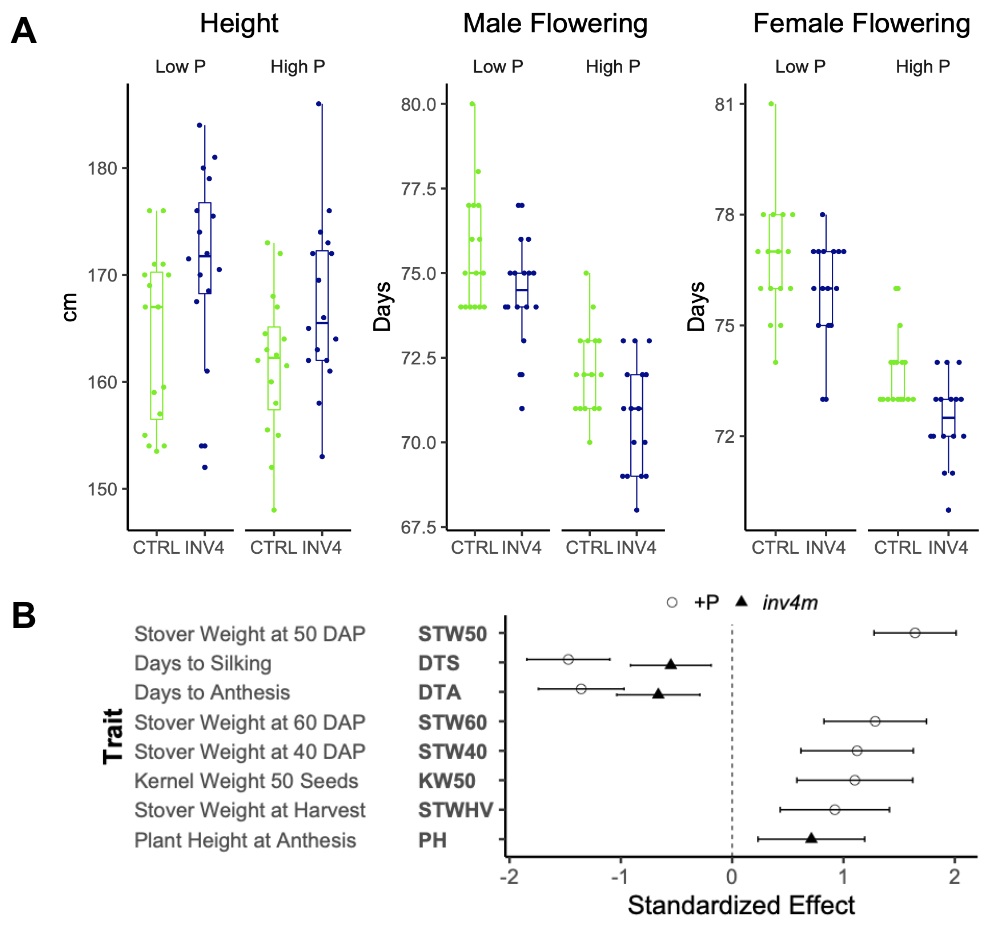
\includegraphics[width=\linewidth]{Chapter-3/figs/effects.png}
\caption[\textit{\invfour} plants flower earlier and are higher independent of phosphorus treatment]{\textit{\textbf{\invfour plants flower earlier and are higher independent of phosphorus treatment}}
% \\\hspace{\textwidth} 
\textbf{(A)} Distribution of traits where \textit{\invfour} genotype has a significant effect. ( Multivariable Multiple regression F test, fdr $<0.05$)
\textbf{(B)} Phosphorus treatment (circle), shows the greatest number of significant effects on traits, and larger absolute magnitude, compared to the \textit{\invfour} effect (triangle). Multivariable Multiple regression effect estimation mean $\pm$ 95 percent confidence interval (whiskers).}
\label{fig::effects}
\end{figure}


\begin{figure}[!ht]

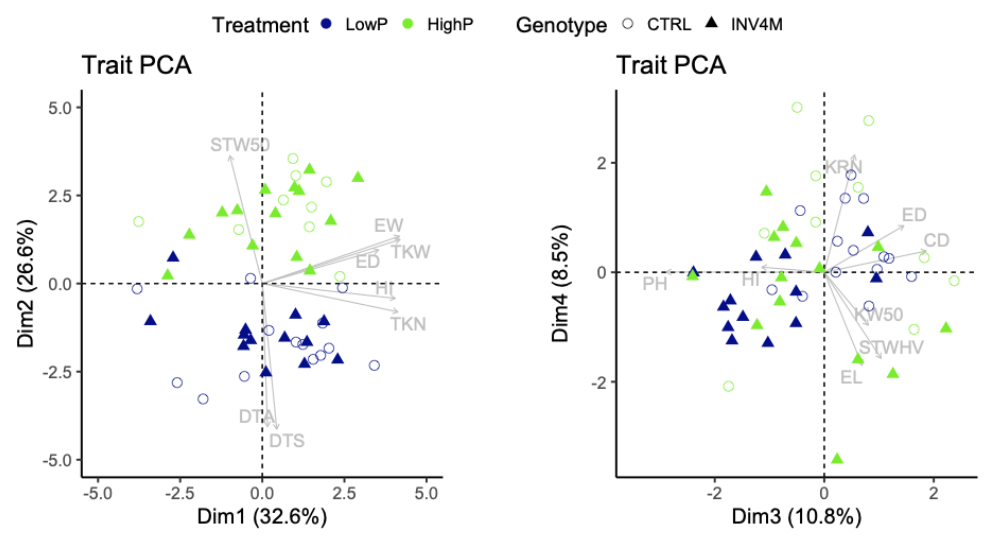
\includegraphics[width=\linewidth]{Chapter-3/figs/traitPCA.png}
\caption[Trait PCA showing that the effect of Phosphorus treatment dominates phenotype differences.]{\textbf{\textit{Trait PCA showing that the effect of Phosphorus treatment dominates phenotype differences.}}
% \\\hspace{\textwidth} 
\textit{Left:} Dim2, whose main contributors are Stover weight at 40 days after pollination, Days to Anhesis, and Days to Silking, sharply separates plants by phosphorus treatment. \textit{Left:} There is a slight separation by \textit{\invfour} genotype along Dim3, and especially along the Ear Diameter projection on this plane}
\label{fig::traitPCA}
\end{figure}

\begin{figure}[!ht]
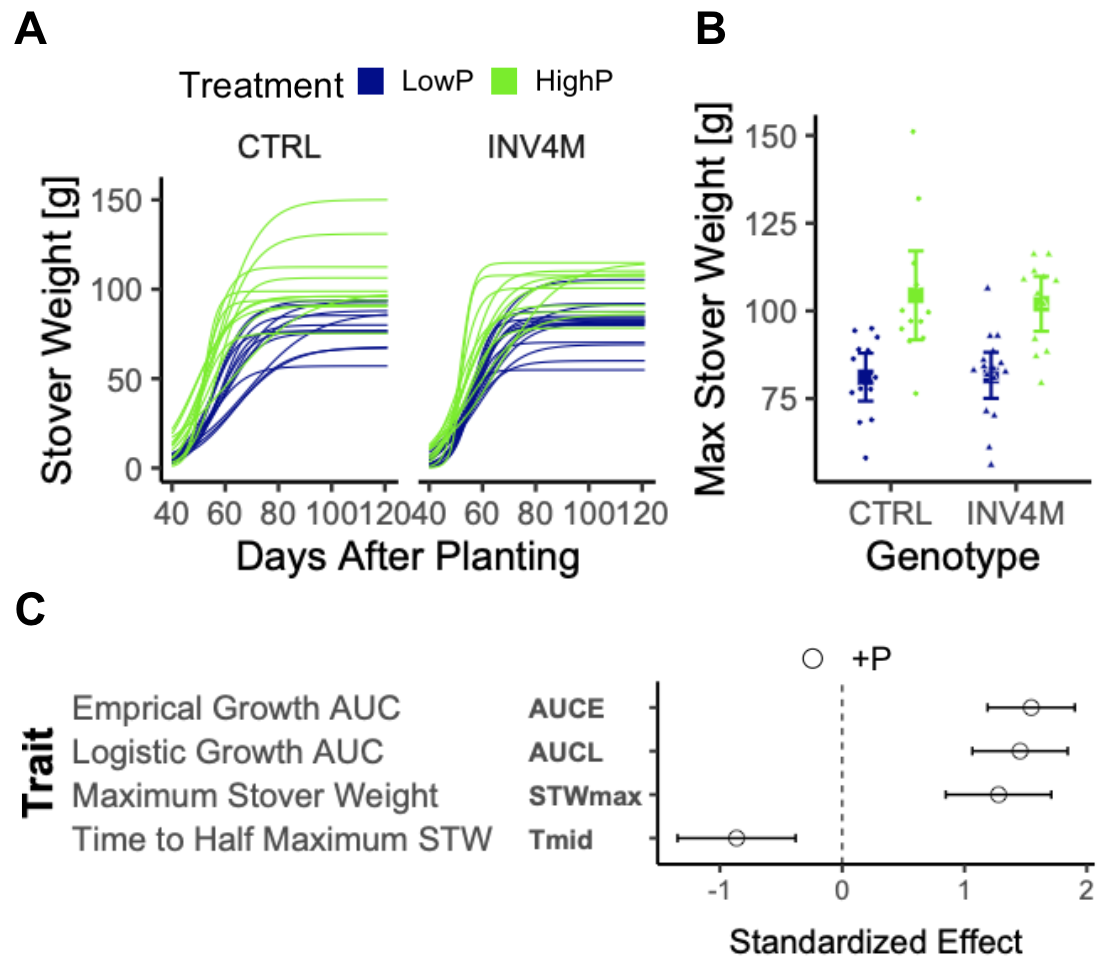
\includegraphics[width=\linewidth]{Chapter-3/figs/growth.png}
\caption[Plant growth curves show effect of phosphorus treatment but no \textit{\invfour} effect]{\textbf{\textit{Plant growth curves show effect of phosphorus treatment but no \textit{\invfour} effect.}}
% \\\hspace{\textwidth} 
\textbf{(A)} Stover dry weight, logistic growth fit curves per field row.
\textbf{(B)} Maximum Stover Weight mean and 95 percent confidence interval.
\textbf{(C)} Multivariable Multiple regression effect estimation mean $\pm$ 95 percent confidence interval (whiskers).
}
\label{fig::growth}
\end{figure}


\subsection{Leaf gene expression shows a marked response to Phosphorus and \invfour, with a single gene responding to \invfour $\times$ P interaction}

Plants showed a remarkable response to phosphorus in their leaf gene expression.
A multidimensional scaling analysis of the gene expression data (\autoref{fig::RNAseq} B) shows an overall response to phosphorus that tends to increase with more basal position of the leaf and is associated with the first dimension. 
The second dimension shows more separation between samples due to leaf position.

After a analysis for the effects of phosphorus treatment in gene expression we see that mir399 is consistently over-expressed from the most apical to the most basal of the sampled leaves.
Gene expression on target genes like SPX transporters was also consistently diminished in high phosphorus, corresponding to the overall expected response to phosphorus.

The phosphorus treatment has a genome-wise effect on gene expression, as shown by the mashr p-values {expression manhattan plots}. We found a total of 7373 differential expressed genes (out of  24249 genes detected in at least one leaf sample), with a distribution mostly consistent with gene density throughout the genome (\autoref{fig::RNAseq} C).
In contrast, the effect of \invfour is mostly detected inside the boundaries of \invfour 
% [I need to genotype the samples  show the actual boundaries  in these plants]
with a RNA-directed DNA polymerase, \textit{Zm00001eb190670} being the most significantly affected gene in the group.
Out of 528 DEGs detected for \invfour 263 genes that showed effect in cis, while 265 genes showed significant differential gene expression in trans between \invfour karyotypes.

% (mean fold value of the two groups, t-test p value (sperate hypothesis for over and under expressed genes?)).

\begin{figure}[!ht]
\centering
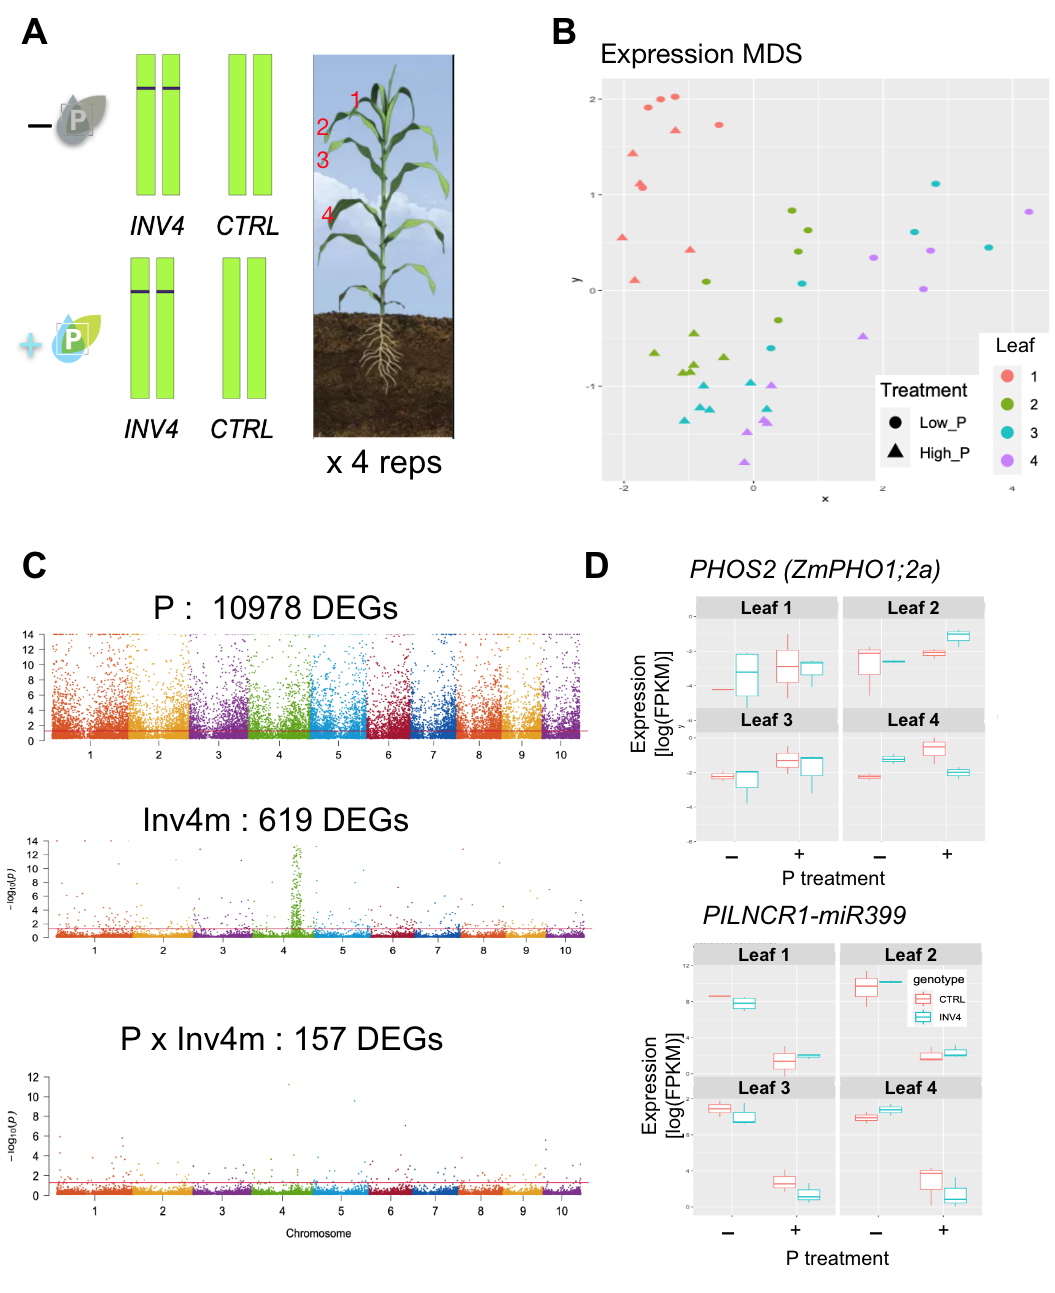
\includegraphics[width=0.95\linewidth]{Chapter-3/figs/RNAseq.png}
\caption[Effect of \invfour, Phosphorus Treatment and Interaction in Gene Expression]{\textit{\textbf{Effect of \invfour, Phosphorus Treatment and Interaction in Gene Expression.}}\\
\hspace{\textwidth} 
\textbf{(A)} Experimental Design.
\textbf{(B)} Gene Expression Multidimensional Scaling. Samples cluster by leaf and P treatment.
\textbf{(C)} Manhattan plots showing statistical significance of differential gene expression between P treatments, \textit{\invfour} genotype and P x \invfour interaction. Vertical lines in the inlay show the reported limits of \invfour \citep{calfee2021-mr}.
\textbf{(D)} \textit{top:} effect of P treatment on the PSR regulator \textit{PILNCR1-miR-399}, and \textit{bottom:} effect of the P x \invfour interaction on the expression of \textit{aldh2}.}
\label{fig::RNAseq}
\end{figure}
\clearpage

However, the variation at \invfour seems to have no major effectnn the gene response to phosphorus.
The \invfour x P interaction t-test (fdr <0.005) shows only one gene with differential response to phosphorus depending on the \invfour karyotype. This gene is found in  near \invfour, but outside previously reported limits (\autoref{fig::RNAseq} C).
A single gene \textit{aldh2}, 3 Mb upstream of the reported \invfour limit,  shows a different response  to phosphorus depending on the \invfour genotype. In phosphorus defficiency \textit{aldh2} overexpresses in  the CTRL plants, but it is not responsive in the \invfour plant (\autoref{fig::RNAseq} D).



\section{Discussion}

 The effect of \invfour in flowering time, previously reported as an association study hit \citep{romero_navarro2017-cn, barnes2022,gates2019-xu}, was confirmed by the experimental introgression of the isolated inverted haplotype into a single genetic background (B73). 
 Additionally, we observed that in this particular background \invfour, increases plant height at flowering.
 These two effects are additive with the corresponding effects of phosphorous treatment. 
 The response of the experimental plants to phosphorus was observed in more phenotypes and was of greater magnitude than the effect of \invfour (\autoref{fig::effects}). 
 In phosphorus deficiency the plants showed delayed growth as both a later time to half maximum stover dry weight and longer times to male and female flowering.
 Plants grew smaller in the absence of phosphorus, accumulated less vegetative biomass as stover dry weight at harvest, and had smaller kernels (KW50) (\autoref{fig::effects}).
 No significant \invfour $\times$ P interaction was detected ($\beta$ t-test, $\textrm{fdr} > 0.05$ for all phenotypes).
 Regarding leaf transcriptome, the master regulator of the phosphorus starvation response  \textit{PILNCR1-mir399} was over-expressed in phosphorus deficiency independent of \invfour genotype (\autoref{fig::RNAseq} D). 
 \textit{PILNCR1-mir399} has been reported to be overexpressed in low phosphorus, and in particular it is more responsive in P-inefficient than in P-efficient genotypes \citep{du2018}.
 B73 has been reported to be phosphorus inefficient with respect other inbreds like Mo17\citep{zhu2005}, and has been selected for yield under high input agriculture compared with traditional varieties such as Mi21. However, \textit{PILNCR1-mir399} response to phosphorus in the experimental plants show no dependency on the variation at \invfour. 
 This suggests that the master regulator phosphorus starvation response is not regulated by \invfour in the experimental conditions. 
 An alternative explanation, is that the experimental P limitation was not hard enough to show a genotype-dependent difference in response. 
 No observable difference in anthocyanin accumulation, or lower leaf senescence in response to phosphorus deficiency in the plant leaves was observed in the field.

We observed a clear over-representation of nitrogen-associated biological processes and metabolic pathways in the 7373 genes responsive to phosphorus treatment (Fisher exact test GO over representation adjusted FDR < 1e-6). 
However, when we reduce the list to the top 1000 most significant, the over-represented gene processes and terms are more related to phosphorus (Fisher exact test GO over representation adjusted FDR < 1e-6). 
This suggests that the genes that show the greater and/or more consistent effect  have phosphorus-associated functions while nitrogen-related genes are making significant but smaller adjustments in expression, maybe reflecting cross-talk between phosphorus and nitrogen homeostasis\citep{torres-rodriguez2021}.
I could not find signals of photosynthesis or carbohydrate over representation in the \invfour responsive to inversion karyotype, as was previously found in response to cold \citep{crow2020}.
 
Overall, there is no evidence from this transcriptome experiment that \invfour contributes to local adaptation to phosphorus, in the sense that its adaptive contribution does not depend on phosphorus amount in the the soil.
However, it is clear that \invfour plants flower earlier and are taller irrespective of the phosphorus status.

\newpage

\printbibliography[heading=subbibnumbered, title=References]

